\documentclass[border=5pt, tikz]{standalone}
\usepackage{pgfplots}
\begin{document}
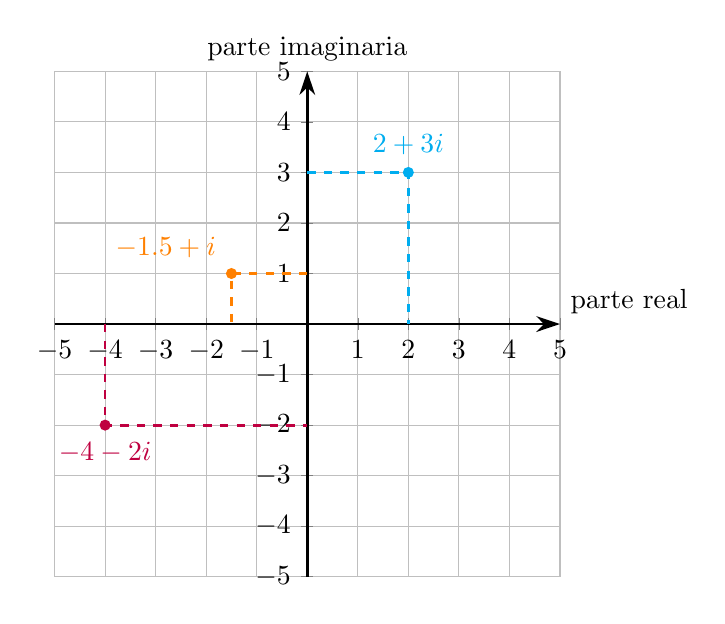
\begin{tikzpicture}
\tikzset{every picture/.append style={line width=1pt}}
\tikzset{vertex/.style={circle, fill, inner sep=0pt,minimum size=4pt}}
\usetikzlibrary{arrows.meta} % For Stealth arrow
\pgfplotsset{compat=1.11}    % Make "axis cs" default axis coord system.

\begin{axis}[ 
, axis lines = middle
, width=8cm
, height=8cm
, xlabel = {parte real} 
, ylabel = {parte imaginaria} 
, xmin=-5
, xmax=5
, ymin=-5
, ymax=5
, xtick={-5,-4,...,5}
, ytick={-5,-4,...,5}
, grid
, x label style={above right}   
, y label style={above}
, axis line style=-{Stealth[length=3mm,width=2mm]}
]
\draw[dashed, purple] 
    (-4,0) |- node[vertex, label={below:$-4-2i$}] {} 
    (0,-2);

\draw[dashed, cyan] 
    (0,3) -| node[vertex, label={above:$2+3i$}] {} 
    (2,0);

\draw[dashed, orange] 
    (0,1) -| node[vertex, label={above left:$-1.5+i$}] {} 
    (-1.5,0);
\end{axis} 
\end{tikzpicture}
\end{document}